\documentclass{beamer}
\usetheme{gvsuthesis}
\usepackage[style=ieee,backend=bibtex,url=false]{biblatex}
\addbibresource{references.bib}


\title{Design of a UAV Perching Device for Detection and Grasping}
\author{Wyatt Barber}
\institute{Grand Valley State University}
\date{Nov. 19, 2026}


\begin{document}

\frame{\titlepage}

\begin{frame}{Agenda}
    \tableofcontents
\end{frame}


\section{Introduction}

\begin{frame}{Background}
    \begin{columns}[T]        
        \begin{column}{0.49\textwidth}
            Drone Perching:
            \begin{itemize}
                \item Form of multi-modal locomotion \cite{meng_aerial_2022}.
                \item Mixes powered flight with unpowered and stationary rest \cite{meng_aerial_2022}.
            \end{itemize}
        \end{column}
        
        \begin{column}{0.49\textwidth}
            \centering
            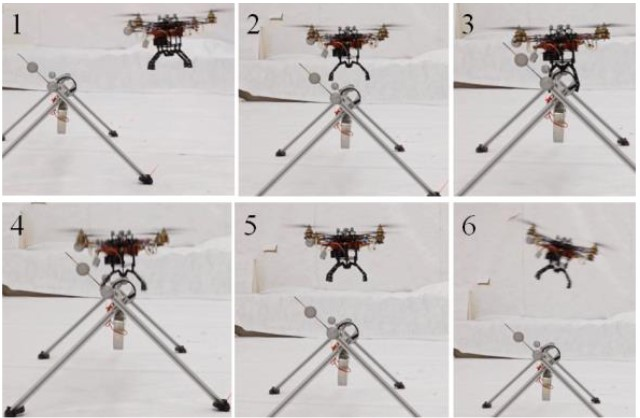
\includegraphics[width=\textwidth]{screenshots/claw.jpg}
            {\small Adapted from \cite{chi_optimized_2014}.}
        \end{column}
    \end{columns}    
\end{frame}

\begin{frame}{Significance}
    \begin{itemize}
        \item Perching has applications in data collection and environmental monitoring, infrastructure inspection, and disaster response
        \cite{liu_perching_2022,kirchgeorg_hedgehog_2022,hoang_autonomous_2024,kitchen_design_2020,liu_mini-drone_2023,seiber_tracking_2018}.
        \item Few real-world implementations found.
        \item Methods of detecting and grasping perches that are affordable and easy to implement make perching behaviors more accessible to researchers.
        \item Affordability and accessibility accelerate implementation of new perching applications. 
    \end{itemize}
\end{frame}

\begin{frame}{Objectives}
    \begin{itemize}
        \item Design a perch detection method using low-cost and open-source components.
        \item Design a low-cost, simple to fabricate grasping device.
        \item Verify the reliability and accuracy of the design.
    \end{itemize}
\end{frame}


\section{Review of Literature}

\begin{frame}{Applications of Perching}{Infrastructure Inspection}
    \begin{columns}[T]        
        \begin{column}{0.49\textwidth}
            \begin{itemize}
                \item Drones may make inspecting power lines safer and faster \cite{chen_automatic_2018}.
                \item Perching drones could extend their mission time 
                    by perching and charging from power lines \cite{hoang_autonomous_2024,kitchen_design_2020}.
            \end{itemize}
        \end{column}        
        \begin{column}{0.49\textwidth}
            \centering
                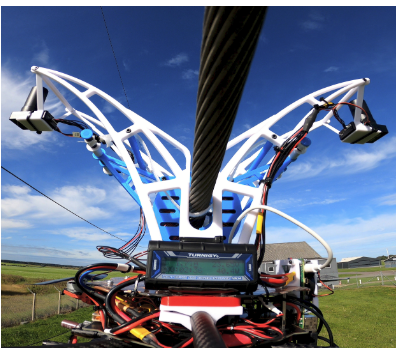
\includegraphics[width=\textwidth]{screenshots/clasp-2.png}
                {\small Adapted from \cite{hoang_autonomous_2024}.}
        \end{column}
    \end{columns}    
\end{frame}

\begin{frame}{Applications of Perching}{Environmental Monitoring}
    \begin{columns}[T]        
        \begin{column}{0.49\textwidth}
            \begin{itemize}
                \item Drones have been proposed to study inaccessible forest canopies,
                    replacing hazardous climbing or costly cranes
                    \cite{kirchgeorg_hedgehog_2022,parker_access_1992,nakamura_forests_2017}
                \item Perching can mitigate disruptive noise \cite{jenni-eiermann_unmanned_2017,bennitt_terrestrial_2019}.
                \item Practical use may be limited to very extreme scenarios, drones for depositing 
                    and retrieving sensors may find wider use \cite{dohm_notitle_2024, ostaszewski_notitle_2024}.
            \end{itemize}
        \end{column}        
        \begin{column}{0.49\textwidth}
            \centering
                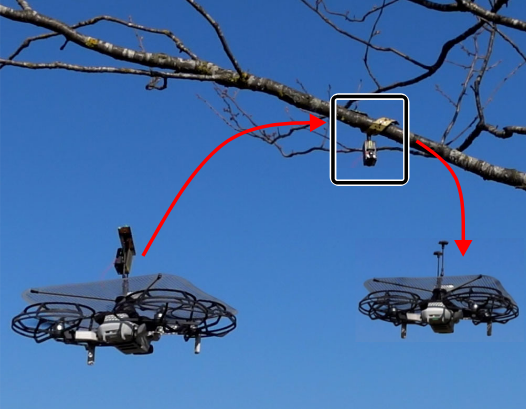
\includegraphics[width=\textwidth]{screenshots/bistable_coil.png}
                {\small Adapted from \cite{geckeler_bistable_2022}.}
        \end{column}
    \end{columns} 
\end{frame}

\begin{frame}{Applications of Perching}{Disaster Response}
    \begin{columns}[T]        
        \begin{column}{0.49\textwidth}
            \begin{itemize}
                \item Drones could rapidly deploy sensors to track boundaries of toxic plumes \cite{seiber_tracking_2018}.
                \item Perching behavior could extend the mission time of this sensor fence, while keeping rapid 
                    deployment and reconfigurability \cite{liu_perching_2022}.
            \end{itemize}
        \end{column}        
        \begin{column}{0.49\textwidth}
            \centering
                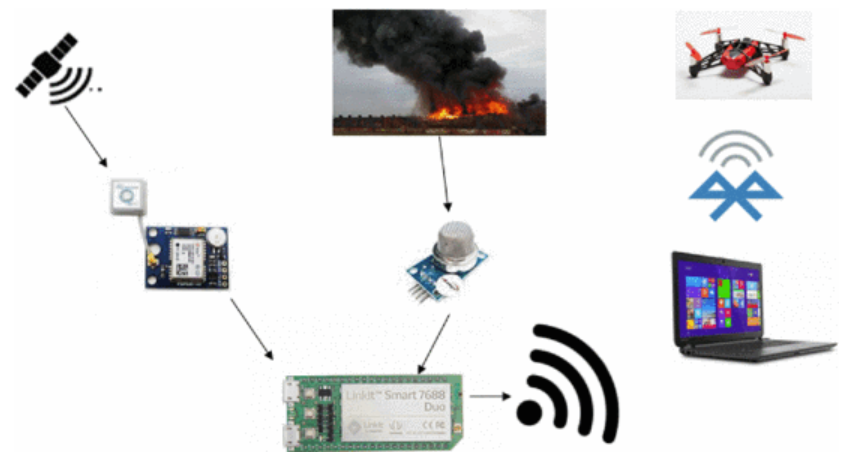
\includegraphics[width=\textwidth]{screenshots/plume-monitor.png}
                {\small Adapted from \cite{seiber_tracking_2018}.}
        \end{column}
    \end{columns} 
\end{frame}

\begin{frame}{Modes of Perching}
    \begin{columns}[T]        
        \begin{column}{0.49\textwidth}
            Meng et al. identified 3 primary modes of drone perching \cite{meng_aerial_2022}:
            \begin{itemize}
                \item<1-> Grasping 
                \item<2-> Embedding
                \item<3-> Attaching
            \end{itemize}
        \end{column}
        
        \begin{column}{0.49\textwidth}
            \centering
            \only<1> {
                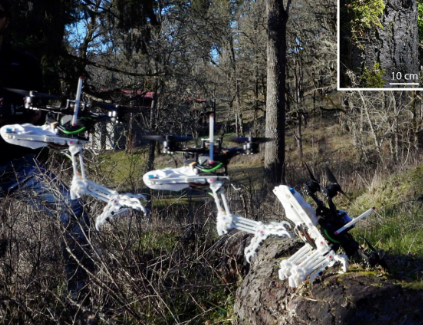
\includegraphics[width=\textwidth]{screenshots/birdclaw.png}
                {\small Adapted from \cite{roderick_bird-inspired_2021}.}
            }
            \only<2> {
                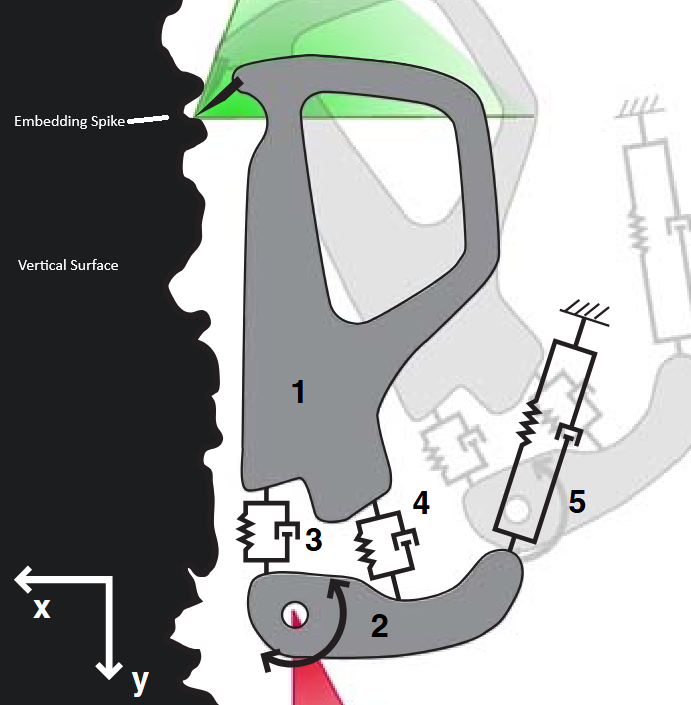
\includegraphics[width=\textwidth]{screenshots/fixedwing-spines.png}
                {\small Adapted from \cite{lussier_desbiens_landing_2010}.}
            }
            \only<3> {
                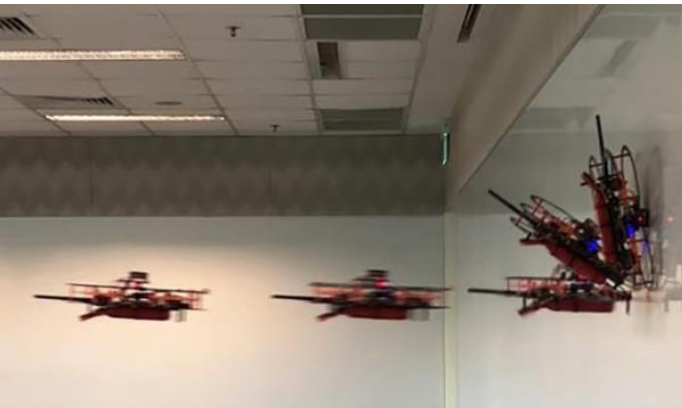
\includegraphics[width=\textwidth]{screenshots/electromagnetic.png}
                {\small Adapted from \cite{liu_perching_2022}.}
            }
        \end{column}
    \end{columns}    
\end{frame}

\begin{frame}{Methods of Perch Detection}
    \begin{columns}[T]        
        \begin{column}{0.49\textwidth}           
            \begin{itemize}
                \item<1-> Kominami et al. designed a method based on depth profiles between 
                    edges in the RGB image \cite{kominami_detection_2023}.
                \item<2-> von Frankenberg and Nokleby's method detects cylindrical shapes directly 
                    in point clouds with a RANSAC method \cite{von_frankenberg_detection_2020}.
                \item<3-> Hoang et al used a radar module paired with a camera to detect power lines \cite{hoang_autonomous_2024}.
            \end{itemize}
        \end{column}
        
        \begin{column}{0.49\textwidth}
            \centering
            \only<1> {
                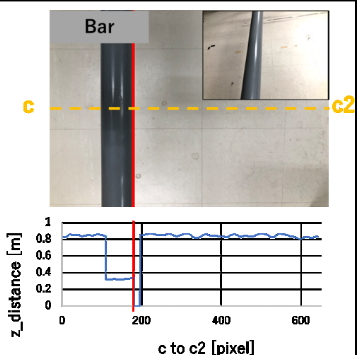
\includegraphics[width=\textwidth]{screenshots/kominami-detect.png}
                {\small Adapted from \cite{kominami_detection_2023}.}
            }
            \only<2,3> {
                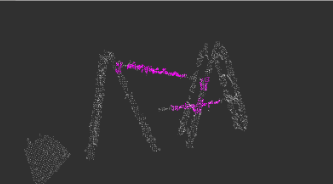
\includegraphics[width=\textwidth]{screenshots/frankenburg-detect.png}
                {\small Adapted from \cite{von_frankenberg_detection_2020}.}
            }
        \end{column}
    \end{columns}   
\end{frame}


\section{Methods}


\section{Results}


\section{Conclusions and Future Works}



\begin{frame}[allowframebreaks]{References}
    \renewcommand*{\bibfont}{\small}
    \printbibliography[heading=none]
\end{frame}


\end{document}